\documentclass[12pt]{article}
\usepackage{graphicx}
\usepackage[utf8]{inputenc}
\usepackage{relsize}
\usepackage{url}
\usepackage{color}
\usepackage{amsmath}
\usepackage{amsthm}
\usepackage{amsfonts}
\usepackage{amssymb}
\usepackage{mathtools}
\usepackage{graphicx}
\usepackage{amsmath}
\usepackage{siunitx}
\usepackage{caption}
\usepackage{graphicx}
\usepackage{relsize}
\usepackage{xparse}
\usepackage{url}
\usepackage{color}
\usepackage{amsmath}
\usepackage{amssymb}
\usepackage{booktabs,caption}
\usepackage[flushleft]{threeparttable}

\usepackage[margin=0.5in]{geometry}

\begin{document}
\title{\textbf{ECON 5P04 Panel Analysis: Charitable Giving}}
\author{Claudia Sestili (5835350) \\ Zachary Mesic (5820105) \\ Ifeanyi Adimorah (5770219) \\ Steven Iamarino (5667753)}
\date{\today}
\maketitle

\thispagestyle{empty}
\vfill
\begin{center}
\textbf{BROCK UNIVERSITY}
\break
Master of Business  Economics
\break
Professor Tomson Ogwang

2020
\end{center}

\newpage

A) 
\begin{table}[!htbp] \centering 
\begin{threeparttable}
  \caption{Pooling Model Regression Results} 
  \label{} 
\begin{tabular}{@{\extracolsep{3pt}}lcccc} 
 \toprule
\midrule
\\
Residuals: \\
\hline \\[-1.8ex] 
     Min. &  1st Qu.  &  Median &  3rd Qu.   &   Max. \\
-4.737340 & -0.606864 & 0.056466 & 0.727930 & 3.505346 \\
 & \\ 
Coefficients: \\
\hline \\[-1.8ex] 
       &       Estimate & Std. Error & t-value  & Pr($>|t|$)  \\
(Intercept) & -4.6742194  & 1.2981340 & -3.6007 & 0.0003515 *** \\
income    &   1.0357785  & 0.1289442  & 8.0328 & 7.935e-15 *** \\
price  &      0.4830921  & 0.2077034  & 2.3259 & 0.0204553 *  \\
age     &     1.5472745 & 0.2169547 & 7.1318 & 3.826e-12 *** \\
ms      &    -0.0080364  & 0.1848487 & -0.0435 & 0.9653411   \\
deps   &      0.1753681  & 0.0426421  & 4.1126 & 4.629e-05 *** \\
\bottomrule
	 \end{tabular}
 \begin{tablenotes}
\small
\item \textit{Note:} Signif. codes:  0 ‘***’ 0.001 ‘**’ 0.01 ‘*’ 0.05 ‘.’ 0.1 ‘ ’ 1
\item \ 
\item Total Sum of Squares:    809.35 
\item Residual Sum of Squares: 627.66 
\item R-Squared:      0.22449 
\item Adj. R-Squared: 0.21613 
\item F-statistic: 26.8628 on 5 and 464 DF, p-value: $<$ 2.22e-16 
\end{tablenotes}
  \end{threeparttable}
\end{table}

\begin{table}[!htbp] \centering 
\begin{threeparttable}
  \caption{Individual Fixed Effects Model Regression Results} 
  \label{} 
\begin{tabular}{@{\extracolsep{5pt}}lcccc} 
 \toprule
\midrule
\\
Residuals: \\
\hline \\[-1.8ex]
     Min.  & 1st Qu. &   Median &  3rd Qu.   &   Max. \\
-3.608066 & -0.264850 &  0.030264  & 0.310411 &  2.348169 \\
\\
Coefficients: \\
\hline \\[-1.8ex] 
   &     Estimate & Std. Error &  t-value  & Pr($>|t|$)    \\
income &  0.838810  &  0.111267 & 7.5387 & 2.976e-13 *** \\
price  &  0.366080  &  0.124294 & 2.9453 &  0.003407 ** \\
age   &  0.102249  &  0.208039  & 0.4915 &  0.623338    \\
ms    &  0.199833 &  0.263890 & 0.7573  & 0.449322    \\
deps   & -0.086352  & 0.053483 & -1.6146 &  0.107154  \\
\bottomrule
 \end{tabular}
 \begin{tablenotes}  
\small
\item \textit{Note:} Signif. codes:  0 ‘***’ 0.001 ‘**’ 0.01 ‘*’ 0.05 ‘.’ 0.1 ‘ ’ 1
\item \ 
\item Total Sum of Squares:    221.58
\item Residual Sum of Squares: 191.67
\item R-Squared:      0.13497
\item Adj. R-Squared: 0.029433
\item F-statistic: 13.0445 on 5 and 418 DF, p-value: 8.2159e-12
\end{tablenotes}
  \end{threeparttable}
\end{table} 


\begin{table}[!htbp] \centering 
\begin{threeparttable}
  \caption{Individual Random Effects Model Regression Results} 
  \label{} 
\begin{tabular}{@{\extracolsep{5pt}}lcccc} 
 \toprule
\midrule
\\
Residuals: \\
\hline \\[-1.8ex]
     Min.  & 1st Qu. &   Median &  3rd Qu.   &   Max. \\
-3.820238 & -0.278886 &  0.060427 &  0.371336 &  2.170378  \\
 \\
Coefficients:  \\
\hline \\[-1.8ex]
    &         Estimate Std. & Error & z-value & Pr($>|z|$)    \\ 
(Intercept) & -2.370567   & 1.114863 & -2.1263 &  0.033476 *   \\
income   &    0.852996  &  0.108734  & 7.8448 & 4.337e-15 *** \\
price    &    0.370199  &  0.125398  & 2.9522  & 0.003155 **  \\
age     &     0.277063  &  0.201695  & 1.3737  & 0.169544     \\
ms      &     0.199669  &  0.233954 &  0.8535  & 0.393406     \\
deps   &     -0.036254 & 0.049289 & -0.7355 & 0.462013   \\
\bottomrule
 \end{tabular}
 \begin{tablenotes}    
\small
\item \textit{Note:} Signif. codes:  0 ‘***’ 0.001 ‘**’ 0.01 ‘*’ 0.05 ‘.’ 0.1 ‘ ’ 1
\item \ 
\item Total Sum of Squares:    251.12
\item Residual Sum of Squares: 217.79
\item R-Squared:      0.1327
\item Adj. R-Squared: 0.12335
\item Chisq: 70.9941 on 5 DF, p-value: 6.3636e-14
\end{tablenotes}
  \end{threeparttable}
\end{table} 
\newpage

B) In a pooled regression model, the data are treated as if there was a single index with no differences among the individual cross section units. The model is typically a poor fit as a result of ignoring the individual heterogeneity. The resulting coefficients indicate that all independent variables are statistically significant except for marital status. The income coefficient is positive and indicates that controlling for all over variables, a one unit increase in income will increase charitable donations by approximately \$1.04 per year. Similarly, a one unit increase in the tax rate will increase donations by approximately \$0.49 per year and being over the age of 65 increases donations by \$1.55 per year relative to individuals under the age of 65. Lastly, the dependant coefficient indicates that each additional dependant increases donations by \$0.17 per year. \\\\
\hspace{\parindent}There exists two main assumptions of the fixed effects regression model. First, the slopes of the regression lines are the same across states and second, the fixed effects captures entirely the time- constant omitted variables. The results indicate that under the fixed effects regression, the variables age, marital status and dependants are no longer statistically significant. Income and tax (price) remain statistically significant and the coefficients indicate that a one unit increase in income will increase charitable donations by approximately \$0.84 per year. Secondly, a one unit increase in the tax rate will increase charitable donations by approximately \$0.37 per year. \\\\
\hspace{\parindent}The random effects model is an alternative to the fixed effects model. In a random effects model, each individual effect is modelled as a random drawing from a probability distribution with mean 0 and constant variance. There are two main components of this model. First, there exists a random intercept term which measures the extent to which an individuals intercept differs from the overall intercept. Second, there is a "traditional" random error term that varies across individuals and across time. The coefficients when using the random effects model are similar to the results when using the fixed effects model. The age, marriage and dependent variables remain insignificant while income and price remain statistically significant. On average, a one unit increase in income will increase charitable donations by \$0.85 and a one unit increase in the tax rate will increase charitable donations by \$0.37.\\

C) As reported in Table 4, the quasi-within transformation parameter $\theta$ is equal to .7758. The estimate is closer to the fixed effects model due to the value being closer to 1. The random effects model lies between the classical pooling model and the fixed effects model which take on values closer to 0 and 1, respectively. Therefore, a value closer to 0 would indicate that the classical pooling model would be a better fit to the data. \\

 \begin{table}[!htbp] \centering 
\begin{threeparttable}
  \caption{Oneway (Individual) Random Effects Model using Swamy-Arora's Transformation} 
  \label{} 
\begin{tabular}{@{\extracolsep{5pt}}lcccc} 
 \toprule
\midrule
\\
Effects: \\
\hline \\[-1.8ex]
      &           var & std.dev & share & \\
$\hat\sigma_\epsilon^2$ (idiosyncratic): & 0.4585 &  0.6772 & 0.346 & \\
$\hat\sigma_v^2$ (individual):  &  0.8666 & 0.9309 & 0.654 & \\
\\
$\theta$: & 0.7758 & &  & \\
\bottomrule
 \end{tabular}
 \begin{tablenotes}    
\small
\item \textit{Notes:} 
\item
\item plm(formula = charity ~ income + price + age + ms 
\item + deps, data = df, model = "random")
\item
\item Balanced Panel: n = 47, T = 10, N = 470
\end{tablenotes}
  \end{threeparttable}
\end{table} 
\newpage 

D) An F-Test was conducted by comparing the unrestricted, fixed effects regression using dummy variables and the restricted, classical pooling regression to determine which model is a better estimator of the data. The relevant null hypothesis states that there are no fixed effects which implies that the dummy variables that produce the varying intercepts are not statistically significant. In contrast, the relevant alternative hypothesis states that fixed effects exist and therefore, the varying intercepts that result from the fixed effects regression are statistically significant. The test results are as follows: 

\begin{flushleft}
F(5, 464) = 26.8628 $>$ 1.14
\break
F(5, 464) critical value = 1.14 at 5\% significance level.
\end{flushleft} 

At the 5\% significance level, the CV = 1.14. Evidently, the resulting f-statistic is greater than the critical value and therefore, we reject the null hypothesis in favour of the alternative. To conclude, the fixed effects model is the preferred model for our data set.\\

E)  The Breusch- Pagan test is commonly utilized to test for heteroskedasticity. Specifically, it is used to test whether the random effects model or classical pooling model is better suited to the dataset. The relevant null hypothesis states that the variance of the individual effects model equals zero and therefore, the pooled model is the same as the random effects model. As a result, the pooling model is preferred. In contrast, the alternative hypothesis states that the variance of individual effects model is greater than zero and therefore, random effects do exist. The test results are as follows:

\begin{flushleft}
Breusch-Pagan Test for Heteroskedasticity (Using Gretl):
\break
Test statistic: LM = 32.2872
\break
with p-value = P(Chi-square(5) $>$ 32.2872) = 5.21172e-06
\end{flushleft}

The resulting Breusch-Pagan test statistic is 32.2872. This value corresponds with a p-value of approximately zero and therefore, we reject the null hypothesis in favour of the alternative and the random effects model is the preferred model. \\

F) The Hausman Test is often described as a test for model mispecification and in panel data analysis, it is used to choose between a fixed effects model or a random effects model. Specifically, the test is used to determine if there exists a correlation between the unique error term and the regressors in the model. The relevant null hypothesis states that the preferred model is the random effects model and that no correlation exists between the two separate models. In contrast, the alternative hypothesis states that the random effects estimator is inconsistent and therefore, the consistent and efficient fixed effects model is preferred. The test results are as follows: 
\begin{flushleft}
Hausman Test (Using R):
\break
data:  charity $\sim$ income + price + age + ms + deps
\break
chisq = 19.245, df = 5, p-value = 0.00173
\end{flushleft}
As reported above, the resulting Hausman test statistic is 19.245 and has a corresponding p-value of .00173. Since the p-value is less than the 5\% significance level, we reject the null hypothesis in favour of the alternative. Therefore, the error terms are found to be correlated with the regressors and the fixed effects model is the appropriate estimator. \\

G) Based on the test results above, we conclude that the fixed effects model is most appropriate for our data set. Although the Breusch Pagan test determines that the random effects model is the appropriate estimation relative to the classical pooling model, the fixed model is determined to be most appropriate when using the Hausman and F-Tests. Intuitively, this result makes sense because each individual effect is evidently not random.\\

H) The fixed effects model includes a variable that captures the factors that affect the cross section units equally at a given time but do not vary over time. In this model, the subjects are used as their own controls and therefore, their effects are fixed.  Age and marital status are both time-variant variables that are likely to have time-varying effects. Consequently, the age variable is likely retained because as an individuals age varies over time, their maturity and life experiences are likely to influence the size of the donation that they are willing to make. Secondly, marital status is included because one’s marital status might adjust from one time period to the next and therefore the effects are not “fixed”. To conclude, neither age or marital status are fixed or constant. \\

I)  Due to the dimensions of the panel, the existence of unit roots is unlikely. Specifically, there is a relatively small number of years relative to the number of observed individuals. Heterogeneous and homogeneous cases can be tested using first and second generation unit root tests, respectively. The primary difference between the two cases is that the first generation test was developed based on an assumption of cross section independence where as the second generation test allows dependence to prevail across the different units in the panel. To test if there exists a unit root for some or all of the individuals, we conduct the Levin- Lin Chi and IPS tests and obtain p-values less than \num{2.2e -16}. As a result, we reject both of the null hypotheses which state that a unit root exists in favour of the alternatives which implies trend stationarity in the homogenous case. This result is intuitive as income is known to increase with job experience over time. To conclude, the two tests provide evidence that unit roots do not exist. \\\\
Cointegration refers to a relationship between non-stationary, unit root processes (Escudero 20). As we previously concluded, unit roots do not exist within our data and therefore, cointegration is of minimal concern. The variation between the time and individual dimensions provides further evidence on the minimal likelihood of conitergation existing within the dataset. Although there exists many tests for panel cointegration, the most popular is the Pedroni test which can be conducted with or without a constant and/or time trend and would provide evidence against the existence of cointegration within our data. Lastly, there is also minimal worry about autocorrelation due to the dataset being a micro panel. \\\\

J) Adding a lagged-charity variable is a mechanism known as first differencing. First differencing is an approach used to address the problem of omitted variables which results in unnoticed heterogeneity. Dynamic panel data models contain one or more lagged dependant variables and first differences are used to eliminate the individual effects (heterogeneity). Specifically, an instrumental variable for the endogenous first differenced lagged values of the dependant variable are used. This instrument should be correlated with the first differenced lagged values of the dependant variable but uncorrelated with the first differenced error.\\
\break
K) Fixed effects and random effect estimators would be inappropriate to estimate the modified regression parameters discussed in the previous section due to the potential for Nickel bias. This bias results from the demeaning method through which the mean charitable contribution of the individuals as well as the mean of the independent variables are subtracted from each measurable characteristic/variable, establishing a correlation between the regressors and error. In the presence of correlation, the random effects estimator will be biased as proven by the Hausman's test for random effects. Therefore, the demeaning procedure produces regressors that cannot be expressed independently of the error term.\\
\newpage
L) The following coefficients were estimated using the Arelland-Bond Linear Dynamic Panel.
\begin{figure}[h!]
\begin{center}
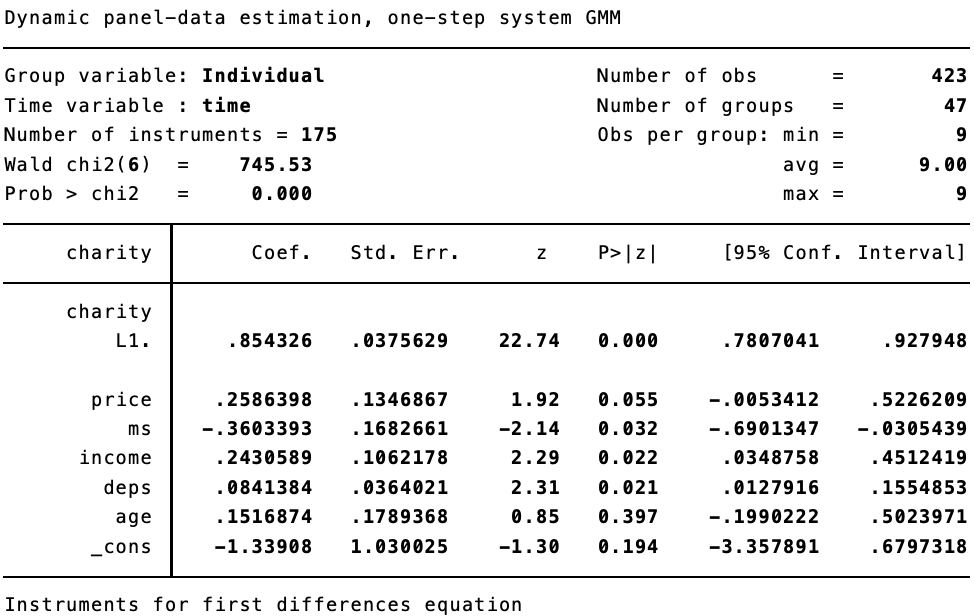
\includegraphics[scale=0.85]{GMM.png}
\label{}
\caption{Arelland-Bond GMM regression results.}
\end{center}
\end{figure}
\break
M) Generalized Moments Method (GMM) introduces an increasing number of instruments when the panel time factor is increased. The estimator is most accurately utilized when the time factor is less than the number of observations. Application of GMM can ultimately become impossible with a broad time dimension.The GMM estimator can be utilized when there exists a large number of time factors and small number of observations however, it is not recommended due to problems associated with a large presence of instrumental variables. Since this particular panel has a small time dimension of 10, this is not a problem. However, if the time factor was high it could possibly fail to implement either of the three GMMs.\\
\break
N) Generalized Moment Method (GMM) and Method of Moments (MOM) are both general for estimating parameters of statistical models. As the name suggests, GMM is a generalization of MOM. The difference between GMM and MOM lies within the definition under which each method should be used. The MOM is a consistent but inefficient estimator that is used when the number of parameters in the model is equal to the number of moment conditions. However, the Generalized Moments Approach is used when the number of parameters exceeds the number of measurements, which is always the case in econometric modelling. Under GMM, the parameter vector is calculated by minimising the sum of the differences in squares between population and sample moments, using the variances of the moments as a metric. This would be considered as the minimum variance estimator.\\


\Large{References}
\begin{flushleft}
\begin{itemize}
\small
\item Escudero, Walter."A Primer on Unit Roots and Cointegration." Econometria, 18 March 2000,
\break
 http://www.depeco.econo.unlp.edu.ar/wp/wp-content/uploads/2017/05/docen3.pdf.
\break
\item Ogwang, T. (2020, March 9). Panel Data Econometrics presented at Brock University in ECON 5P04, St.Catharines.
\break
\end{itemize}
\end{flushleft}
\end{document}





































































\end{document}